% This file was created with tikzplotlib v0.10.1.
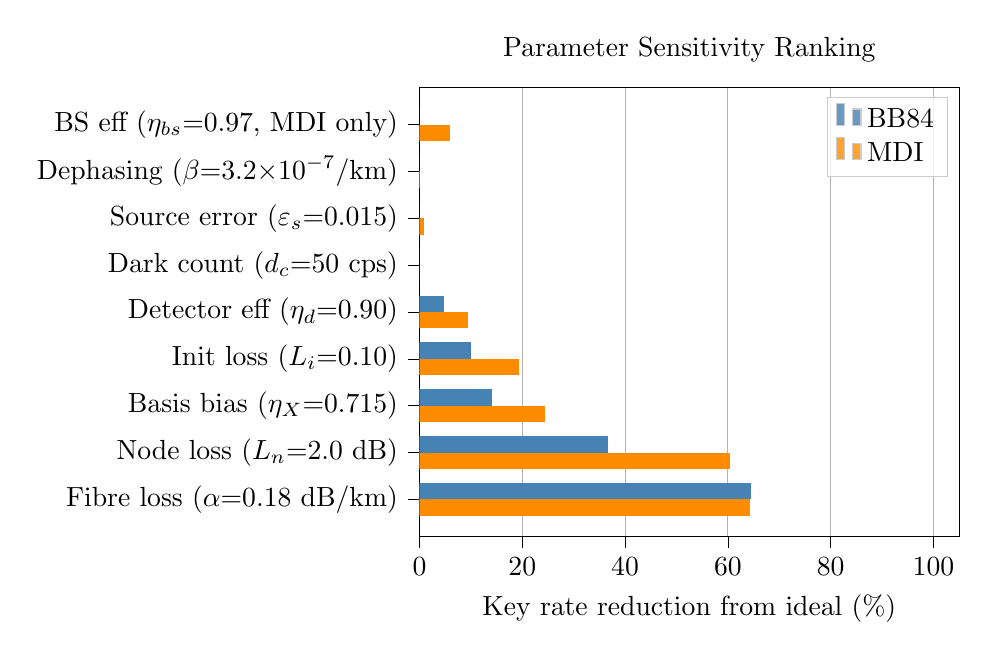
\begin{tikzpicture}

\definecolor{darkgray176}{RGB}{176,176,176}
\definecolor{darkorange}{RGB}{255,140,0}
\definecolor{lightgray204}{RGB}{204,204,204}
\definecolor{steelblue}{RGB}{70,130,180}

\begin{axis}[
legend cell align={left},
legend style={fill opacity=0.8, draw opacity=1, text opacity=1, draw=lightgray204},
tick align=outside,
tick pos=left,
title={Parameter Sensitivity Ranking},
x grid style={darkgray176},
xlabel={Key rate reduction from ideal (\%)},
xmajorgrids,
xmin=0, xmax=105,
xtick style={color=black},
xtick={0,20,40,60,80,100,120},
xticklabels={
  \(\displaystyle {0}\),
  \(\displaystyle {20}\),
  \(\displaystyle {40}\),
  \(\displaystyle {60}\),
  \(\displaystyle {80}\),
  \(\displaystyle {100}\),
  \(\displaystyle {120}\)
},
y grid style={darkgray176},
ymin=-0.785, ymax=8.785,
ytick style={color=black},
ytick={0,1,2,3,4,5,6,7,8},
yticklabels={
  Fibre loss (\(\displaystyle \alpha\)=0.18 dB/km),
  Node loss (\(\displaystyle L_n\)=2.0 dB),
  Basis bias (\(\displaystyle \eta_X\)=0.715),
  Init loss (\(\displaystyle L_i\)=0.10),
  Detector eff (\(\displaystyle \eta_d\)=0.90),
  Dark count (\(\displaystyle d_c\)=50 cps),
  Source error (\(\displaystyle \varepsilon_s\)=0.015),
  Dephasing (\(\displaystyle \beta\)=3.2\(\displaystyle \times10^{-7}\)/km),
  {BS eff (\(\displaystyle \eta_{bs}\)=0.97, MDI only)}
}
]
\draw[draw=none,fill=steelblue] (axis cs:0,2.77555756156289e-17) rectangle (axis cs:64.5294946585941,0.35);
\addlegendimage{ybar,ybar legend,draw=none,fill=steelblue}
\addlegendentry{BB84}

\draw[draw=none,fill=steelblue] (axis cs:0,1) rectangle (axis cs:36.6642612141226,1.35);
\draw[draw=none,fill=steelblue] (axis cs:0,2) rectangle (axis cs:14.1245331870451,2.35);
\draw[draw=none,fill=steelblue] (axis cs:0,3) rectangle (axis cs:9.99089653237982,3.35);
\draw[draw=none,fill=steelblue] (axis cs:0,4) rectangle (axis cs:4.76313095363528,4.35);
\draw[draw=none,fill=steelblue] (axis cs:0,5) rectangle (axis cs:0,5.35);
\draw[draw=none,fill=steelblue] (axis cs:0,6) rectangle (axis cs:0,6.35);
\draw[draw=none,fill=steelblue] (axis cs:0,7) rectangle (axis cs:0,7.35);
\draw[draw=none,fill=steelblue] (axis cs:0,8) rectangle (axis cs:0,8.35);
\draw[draw=none,fill=darkorange] (axis cs:0,-0.35) rectangle (axis cs:64.2982505208736,0);
\addlegendimage{ybar,ybar legend,draw=none,fill=darkorange}
\addlegendentry{MDI}

\draw[draw=none,fill=darkorange] (axis cs:0,0.65) rectangle (axis cs:60.4751300792335,1);
\draw[draw=none,fill=darkorange] (axis cs:0,1.65) rectangle (axis cs:24.488396179666,2);
\draw[draw=none,fill=darkorange] (axis cs:0,2.65) rectangle (axis cs:19.3556921078872,3);
\draw[draw=none,fill=darkorange] (axis cs:0,3.65) rectangle (axis cs:9.42393301246082,4);
\draw[draw=none,fill=darkorange] (axis cs:0,4.65) rectangle (axis cs:0,5);
\draw[draw=none,fill=darkorange] (axis cs:0,5.65) rectangle (axis cs:0.827683987411012,6);
\draw[draw=none,fill=darkorange] (axis cs:0,6.65) rectangle (axis cs:0.168917406156821,7);
\draw[draw=none,fill=darkorange] (axis cs:0,7.65) rectangle (axis cs:6.03261973054838,8);
\end{axis}

\end{tikzpicture}
